\subsubsection{\textbf{Tree Edit Distance (TREED)}}  
The semantic quality of translated code may depend on its syntax. Until now, abstract syntax trees(AST) is the most widely-use structure in representing the syntax of programming code. Therefore, computing the difference of two ASTs is considered as evaluating syntax difference.
In our study, we apply this idea in measuring the difference between the syntax of reference method and translated method. Given a pair of method in C\# which are need to be compared their syntax, Roslyn[cite here] is used to parse them into ASTs. Then we compute the tree edit distance between two trees using the algorithm Treed described in the paper \cite{algorithm}.
To be more detailed, the tree edit distance is calculated by number of operations (add/delete/replace/move) to make them identical. 

We introduce a formuala to normalize the edit distance so that it can be used conveniently in our proposed method in the next part of the paper. The normalized value is computed as:

  $TREED = 1 -  \frac{TreeEditDistance\left(AST_R, AST_T\right)}{CountNodes \left(AST_R+AST_T\right)}$ 
  
where $TreeEditDistance\left(AST_R, AST_T\right)$ is the editing distance between two trees of referenced method $AST_R$ and the translated method $AST_T$; and the denominator is the total nodes in the tree of both two methods. The value of TREED is from 0 to 1. 

For any two trees, there will always exist at least one editing (such as the one that deletes all nodes of the first tree and inserts all the nodes of the second). Therefore, there will always exist at least one TREED value and the higher value it is, the more similar those trees are.

\begin{figure}[h]
	\caption{Tree Editing Example: In the label of each node, its type is in capital font and its val (if exists) is in normal font}
	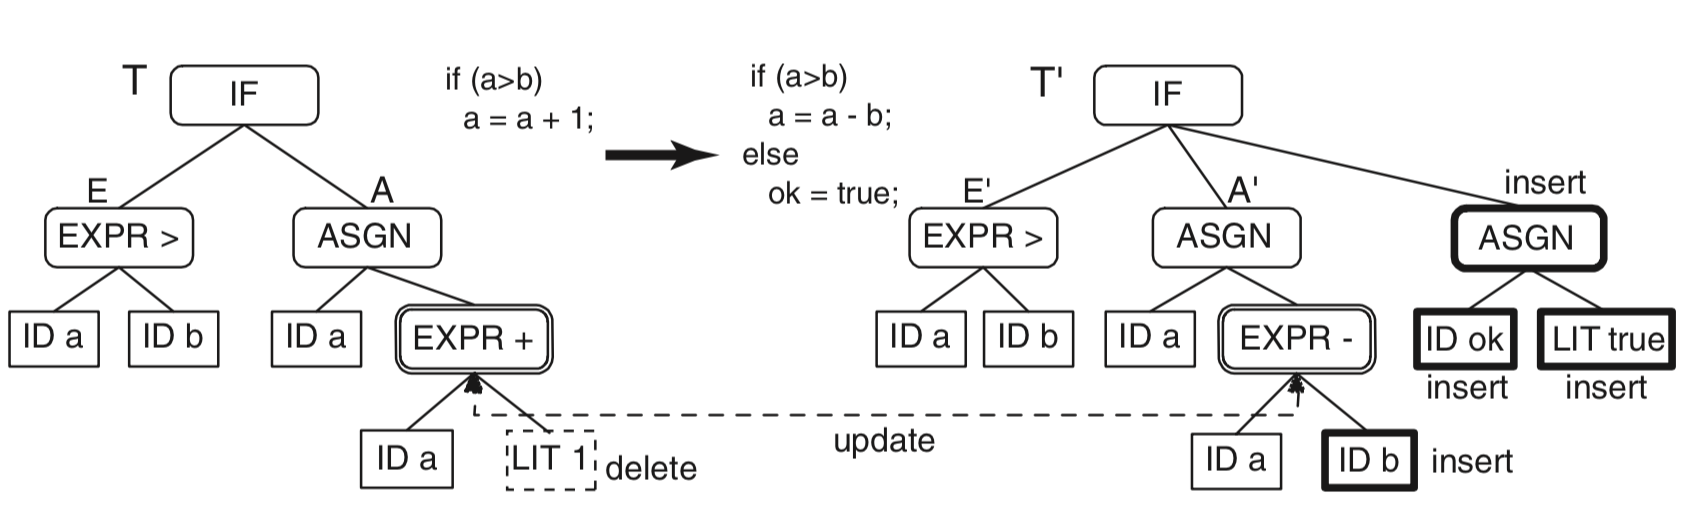
\includegraphics[scale=0.3]{img/treed.png}
	\centering
	\label{fig:treed}
\end{figure}

In the example in Figure \ref{fig:treed}, an \textit{if} statement was edited by modifying the \textit{if} branch and adding an \textit{else} branch. The two trees represent the two versions of a method. An editing consists of one \textit{Delete} (dotted line box), one \textit{Update} (double-line box), and four \textit{Insert} operations (bold boxes). Other nodes (single- line boxes) are either unchanged or moved. Based on the formula TREED, the result of TREED in this case  $TREED = 1 - \frac{1 + 1 + 4}{16}=0.625$




